\section{Introduction}

The past few years have witnessed remarkable progress in the development of Large Language Models (LLMs)~\citep{achiam2023gpt,touvron2023llama}, giving rise to the proliferation of numerous agentic systems~\citep{weng2023agent,shen2024hugginggpt}. For example, ``chain-of-thought'' prompting has unlocked the general-purpose reasoning capabilities of LLMs~\citep{wei2022chain}, and memory mechanisms have been proven effective in simulating human behavioiur~\citep{park2023generative}. These emerging LLM agents have demonstrated astonishing abilities to transform a wide range of tasks, including solving mathematical problems~\citep{romera2024mathematical}, navigating the web~\citep{nakano2021webgpt}, providing financial advice~\citep{ding2024large} and informing medical decisions~\citep{li2024agent}. Therefore, the design of agentic systems plays a crucial role in harnessing the power of LLMs for various downstream applications.

However, current research predominantly relies on manually designed agentic systems tailored for specific tasks, which often depend heavily on expert insight and intensive human labor. Furthermore, these task-specific agent designs frequently struggle to adapt to novel tasks. A few recent studies have explored using LLMs to rewrite and optimize the prompts of existing agents~\citep{fernando2024promptbreeder,yang2024large}. A more recent work introduces the idea to leverage LLMs to search the entire agentic systems defined in code space~\citep{hu2024automated}, enabling the discovery of agents with more flexible prompts, control flows, etc. 
However, these previous approaches are limited in their ability to explicitly recombine the strengths of agentic modules discovered by different researches and located in separate codebases. Another line of research focuses on optimizing the configuration of multi-agent systems~\citep{chen2023agentverse,yuan2024evoagent,li2023metaagents,zhugegptswarm,wang2023unleashing}. These efforts are orthogonal to the optimization of single-agent systems, as they focus more on the role-playing and interaction patterns among multiple agents, rather than the design of agentic modules.

\begin{figure}[!t]
\begin{center}
\vspace{-6mm}
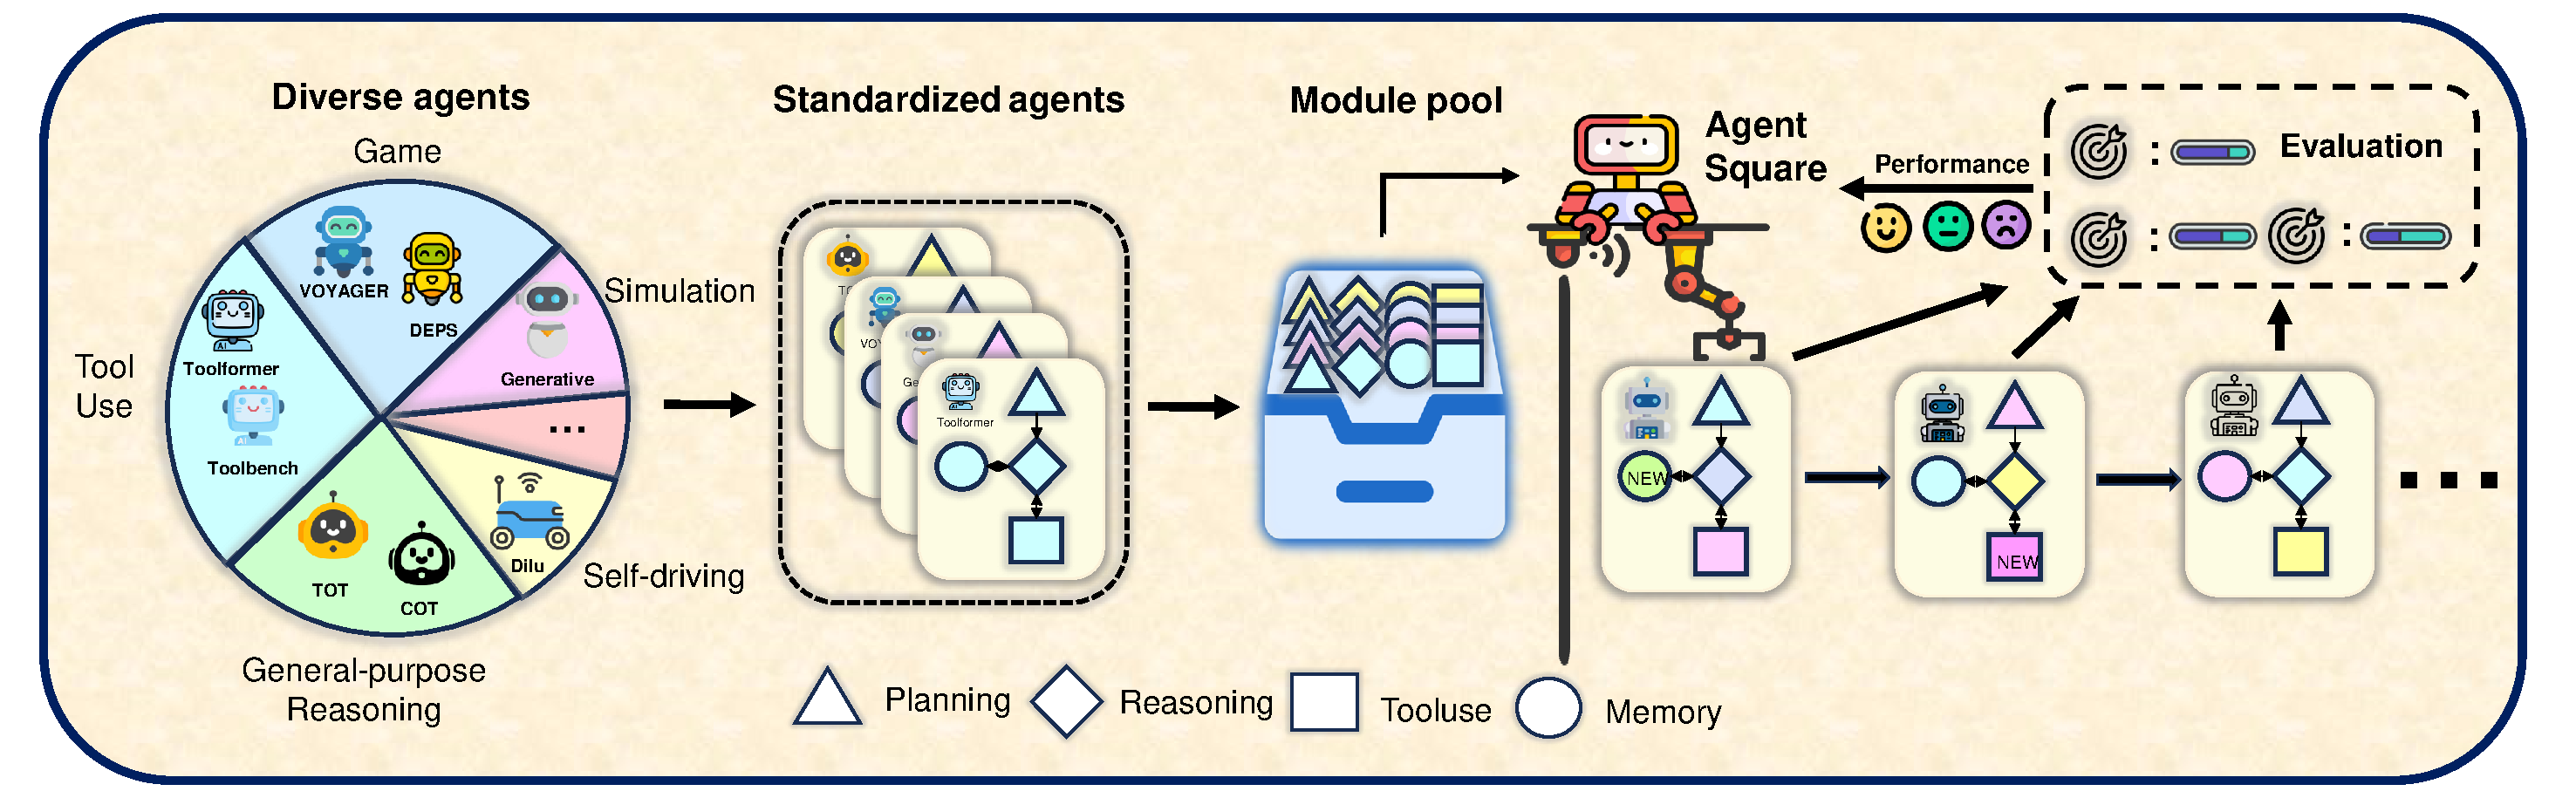
\includegraphics[width=14cm]{Figures/f1.pdf}
\vspace{-6mm}
\caption{AgentSquare is a modular framework for designing and optimizing LLM agents. 
% We first propose a modular design space of LLM agents and extract 4 types of standardized modules including planning, reasoning, tooluse, and memory. Based on this, we design a novel LLM agent search framework to automatically discover good-performing agents.
}
\label{figure1}
\end{center}
\end{figure}

This paper addresses a novel research problem --- \underline{Mo}dularized \underline{L}LM \underline{A}gent \underline{S}earch (MoLAS). The goal is to automatically optimize LLM agent designs by leveraging the experience of published or evaluated modules. Therefore, the core of our work is a modular design space for LLM agents, comprising 4 categories of modules: \emph{Planning}, \emph{Reasoning}, \emph{Tool Use}, and \emph{Memory}. This design space is abstracted from a thorough literature review of existing agentic systems (details provided in Section 2). 
% MoLAS is a guided and constrained searching problem in the modular design space, which is a subset of the entire code search proposed in ADAS. 
It is important to note that our goal is not to propose the most comprehensive, one-size-fits-all LLM agent design space, but rather to demonstrate that our modular design space enables researchers and intelligent search algorithms to fully exploit the potential of prior successful designs. 
MoLAS is a guided and constrained searching problem in the modular design space, which is a subset of the entire code search proposed in ADAS~\citep{hu2024automated}.
However, MoLAS has a nice feature of providing standardized IO interfaces for agent modules, facilitating easy recombination of modules from different agentic systems and hence enabling efficient search for novel agents. Our design space is also highly extensible, allowing new agentic systems to be integrated as plug-in modules. Therefore, it provides a platform to consolidate the collective efforts of the research community on LLM agents. The overview of this work is illustrated in Figure~\ref{figure1}.

Building on this modular design space, we propose a novel LLM agent search framework called AgentSquare. Specifically, AgentSquare optimizes LLM agents through the mechanisms of \emph{module evolution} and \emph{recombination}. The \emph{module evolution} mechanism leverages an evolutionary meta-prompt to explore new modules through prompt-level optimization, which jointly models task descriptions, existing modules, and the performance of evaluated modules. Besides, the \emph{module recombination} mechanism performs module-level optimization by leveraging the reasoning power of LLMs to strategically search for promising module combinations. To reduce the expensive evaluation costs of LLM agents, we further introduce a performance predictor that implements an in-context surrogate model for newly proposed LLM agents, enabling us to skip unpromising candidates and significantly accelerate the search process.

We conduct comprehensive evaluations on six widely adopted benchmarks, covering diverse use cases in web, embodied, tool use and game scenarios. Our experiments show AgentSqaure can discover novel LLM agents that outperform hand-crafted agents across all six benchmarks, scoring an average performance gain of 17.2\% compared to the best known human designs. Besides, AgentSqaure also surpasses other search algorithms in terms of having a steeper optimization trajectory. More importantly, case studies reveal that AgentSquare can provide human interpretable design insights for newly discovered, good-performing agents.

The key contributions of this work are as follows:

\begin{itemize}
    \item We propose a novel modular design space for LLM agents, enabling researchers to easily build on previous successful designs and accumulate new discoveries as a community.
    \item We design the AgentSquare framework that efficiently searches for novel and good-performing LLM agents via the novel mechanism of \emph{module evolution}, \emph{module recombination}, and \emph{performance predictor}.  
    \item Experiments across six diverse tasks show that our method discovers novel LLM agents that outperform all known human designs. Besides, AgentSqaure can generate human interpretable design insights for these novel agents. 
\end{itemize}

